\subsection{Signal Path}
\label{signPath}

The simulated path that the \ac{laser} signal follows is visualized in figure \ref{signPath} on 
page \pageref{signPath}. There are three distinct phases. The first one is the travel of the
signal down through the atmosphere. This is followed by the scattering on the Earth's surface. Finally the
pulse has to travel back up through the atmosphere. This sequence is elaborated on in more
detail below.

The signal originates from the emitter. For each pulse, the emitter position is determined from
a set of Kepler elements. The energy in the pulse is found by distributing the emitter power over a
constant number of pulses of a given duration.

The signal then starts to propagate through the atmosphere. The atmosphere affects the signal in
several manners, but the most important one is the attenuation of the signal. Attenuation is the
only disturbance by the atmosphere taken into account. The pulse energy exponentially decays with
travel distance through the atmosphere. Furthermore also the optical thickness of the atmosphere is taken into account.

Then the intersection of the pulse with the \ac{DEM} is computed. As a simplification in this
process, the intersection of the pulse (i.e., the ray) with a sphere is computed. The sphere has a radius of
the average terrain height of the \ac{DEM} tile plus the Earth radius. Then the ray-sphere
intersection point coordinates are converted into latitude and longitude. These are then used to 
find the actual terrain elevation from the \ac{DEM} and the three-dimensional position.

Then the scattering characteristics are constructed. For this, the terrain normal and the inbound
laser pulse vector are used. The power of the emitted pulse is now distributed over the entire
footprint area of the emitter and then scattered back using the scattering technique described in
section \ref{scatter}. The backscattered energy is computed separately for every receiver satellite.

The reflected pulse now travels back through the atmosphere. More attenuation takes
place along this path. The energy received by the receivers now depends on the receiver aperture. The received
energy can then be converted into photons by dividing the energy received by the energy per photon.

\begin{figure}[ht!]
	\centering
		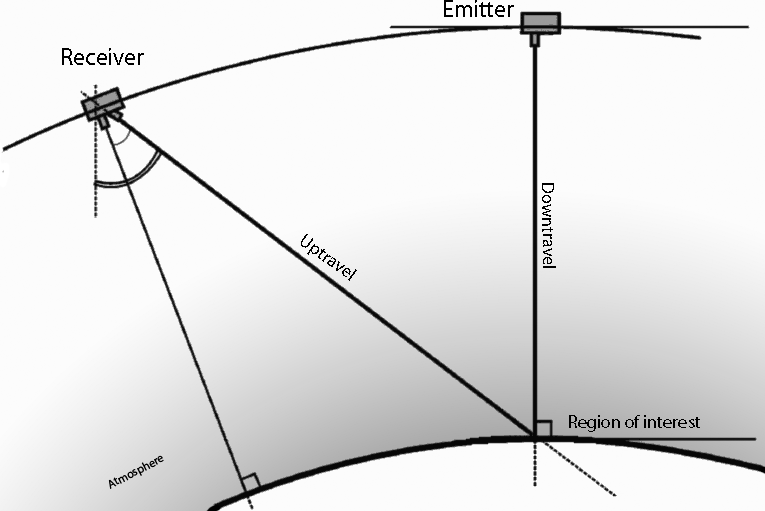
\includegraphics[width=0.8\textwidth]{chapters/img/signalPath.png}
		\label{fig:signalPath}
	\caption{Signal path representation}
\end{figure}